\documentclass[letterpaper, twoside]{article}
\usepackage[utf8]{inputenc}
\usepackage{fullpage}
\usepackage{amssymb}
\usepackage{amsmath}
\usepackage{graphicx}
\usepackage{xcolor}
\usepackage{float}
\usepackage{listings}
\numberwithin{equation}{section}

% Text
\newcommand{\etc}{etc.}
\newcommand{\eg}{e.g.}
\newcommand{\ie}{i.e.}

% Math
\def\bm#1{\mbox{\boldmath{$#1$}}}


\title{Biofilm Model Theory}
\author{Austen, Takumi, Mark, Phil}
\date{}

\begin{document}

\maketitle

\abstract
A one-dimensional biofilm model was created in MATLAB for user specified conditions within a continuous stirred tank reactor. This model utilizes numerical methods to iteratively solve for the diffusion of nutrients into a biofilm over a variable span of time as well as the depletion of nutrients in the tank reactor as they are integrated into the biofilm. Various growth kinetics are used to calculate the respective growth rate of the biofilm and therefore its change in size over time. Considerations for efficiency, convergence, and stability of modeled differential equations have been the prime areas of focus throughout the modeling process to ensure accurate solutions for a wide range of user inputs.

\section{Nomenclature}
\begin{tabular}{c l c}
  Variable & Description & Units\\ \hline
  $\mu$ & Growth Rate & 1/days\\
  $\mu_\mathrm{max}$  & Maximum specific growth rate & 1/days\\
  $\bar\mu$ & Average growth rate & 1/days\\
  $K_\mathrm{m}$ & Monod half saturation coefficient & g/m$^3$\\
  $K_\mathrm{i}$ & Inhibition Coefficient & g/m$^3$\\
  $Y_\mathrm{xs}$ & Biomass yield coefficient on substrate & g$\cdot$g/s\\
  $v_g$ & Biofilm Growth Velocity & m/s\\
  $v_\mathrm{det}$ & Detachment Velocity & m/s\\
  $V$ & Volume &m$^3$ \\
  $Q$	& Flowrate & m$^3$/day\\
  $A$	& Wetted surface area & m$^2$\\
  $S$ & Substration Concentration in tank & g/m$^3$\\
  $S_{\mathrm{in}}$ & Influent substrate concentration &  g/m$^3$ \\
  $S_o$ & Initial bulk fluid substrate concentration in tank &  g/m$^3$ \\
  $S_b$ & Substrate Concentration in biofilm & g/m$^3$ \\
  $x$ & Biomass Concentration in tank & g/m$^3$\\
  $x_o$ & Initial biomass concentration in tank &  g/m$^3$ \\
  $X_b$ & Biomass density in biofilm &  g/m$^3$ \\
  $D_\mathrm{aq}$ & Diffusion coefficient of substrate in water & m$^2$/day \\
  $D_e$ & Effective diffusion coefficient of substrate in biofilm & m$^2$/day \\
  $L_{f}$ & Biofilm thickness & m\\
  $L_L$ & Concentration boundary layer thickness & m \\
  $k_\mathrm{det}$ &	Detachment rate coefficient & 1/(m$\cdot$days)\\
  $z$ & Biofilm Gride Size & m
\end{tabular}

\section{Background}
Multispecies biofilm research has implications in a wide range of fields, from dental plaque growth to gastrointestinal lining in stomachs to structuring the aquatic food chain on the surfaces of rocky riverbeds. Biofilms are the result of respective species of bacteria competing for the substrate within a bulk liquid environment. Bacteria consume nutrients, or substrate, and create biomass, which floats within the liquid until it attaches to a surface. As this biomass attaches to surfaces, they develop an external biofilm which provides protection from the surrounding environment. Following biofilm formation, the detachment phase can begin, and biomass is released to find new surfaces to inhabit.

To simulate biofilm activity and dynamics, a model is sought that incorporates these phenomena: 1) microbial growth 2) substrate consumption/production associated with microbial growth 3) diffusion of dissolved substrates and products into/out of the biofilm 4) activity of both planktonic and biofilm cells, detachment, and 5) system concentrations and flows.

The model constructed here recapitulates the Biofilm Accumulation Model (BAM), developed at the Center for Biofilm Engineering. BAM was itself a version of a model termed BIOSIM that was based on a construct from Oskar Wanner and Willi Gujer.

\section{Code}
This model was created using Matlab, a multi-paradigm programming language utilized across most engineering fields to model and analyze data. This model could be rewritten in a different language such as C, Python, etc. to allow the code to be more accessible in an open source editor format for future changes. This code and all the created files can be accessed through any Git GUI in the public repository created by Dr. Mark Owkes of the mechanical and industrial engineering department at Montana State University. The title of this repository is $BiofilmModel$.

\subsection{Matlab Infrastructure, $BiofilmModel$}
\begin{tabular}{c l c}
  File Name & Description \\ \hline
  biofilmdiffusion\_fd.m & Computes diffusion into biofilm \\
  biofilmTest.m & Runs all tests for code validation \\
  cases.m & Creates "param" structure, hosts all other variables \\
  lf.m & Computes biofilm thickness \\
  MAINDRIVER.m & Organizes and calls all other functions to produce solution \\
  mu.m & Stores all growth rate formulas and calculates growth rate $\mu$ \\
  outputs.m & Inputs all computed data and produces plots for results \\
  tankenvironment.m & Computes concentrations within tank environment \\
\end{tabular}

\subsection{Access}
The file repository can be accessed using any free Git GUI software. Git is a system of project management used to handle large collaborative work involving multiple localities where all the work can be saved and accessed through a remote central cloud. The benefit of this system is that work can be saved and edited remotely until it is ready to be released to the cloud for access and use by all within the project. The two Git systems used most frequently throughout this project were Github and Sourcetree. 

Downloading a system such as Github or Sourcetree will allow any user to search for the repository $BiofilmModel$ and gain access to all the files outlined above. 
  
\section{Tank Environment}
The environment is modeled in this function as a continuous stirred tank reactor (CSTR), with the existence of an inflow and outflow which carries substrate into the bulk liquid, where some initial concentration of biomass already exists.

\begin{figure}[H]
\centering
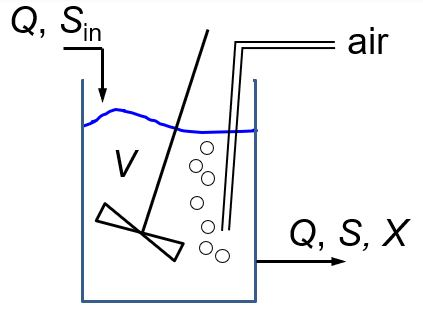
\includegraphics[width=2in]{CSTR_model.jpg}
\caption{Continuous Stirred Tank Reactor}
\end{figure}

The rates of the biomass and substrate are modeled by the following ordinary differential equations with initial conditions $x_j(t=0)=x_{o,j}$ and $S_k(t=0)=S_{o,k}$.
\begin{equation} \label{eq: BiomassEquation}
  \frac{dx_j}{dt} = \mu_j(\bm{S}) x_j - \frac{Q x_j}{V} + \frac{ v_{\mathrm{det}j} A X_{b,j}}{V}
\end{equation}
for $j=1,\dots,N_x$ and 
\begin{equation} \label{eq: SubstrateEquation}
  \frac{dS_k}{dt} = -\sum_{j=1}^{N_x} \frac{\mu_j(\bm{S}) x_j}{Y_{j,k}} + \frac{Q S_{\mathrm{in},k}}{V} - \frac{Q S_k}{V} - \frac{A B_{\mathrm{flux},k}}{V}
\end{equation}
for $k=1,\dots,N_s$.

In order for these differential equations to be solved, they are first into a single vector differential equation
\begin{equation}
  \frac{d \bm{y}}{dt} = \bm{f}(t,\bm{y})
\end{equation}
where 
\begin{equation}
  \bm{y} = [x_1,\dots,x_{N_x}, S_1,\dots,S_{N_S}]^\mathsf{T}
\end{equation}
and 
\begin{equation} \label{eq: ODEpackagef}
  \bm{f}(t,\bm{y}) =\left[ R_{x,1}, \dots, R_{x,N_x},  R_{S,1}, ,\dots, R_{S,N_S}\right]^\mathsf{T}
\end{equation}
where $R_{x,j}$ is the right-hand-side (RHS) of Eq.~\ref{eq: BiomassEquation} and $R_{S,k}$ is the right-hand-side (RHS) of Eq.~\ref{eq: SubstrateEquation}.

A low order Runge-Kutta Method based off the structure of ODE23, an intrinsic Matlab function, is used to discretize and solve the packaged differential equations in this function. The Runge-Kutta numerical method calculates the slope of function at three points between each step of the iteration process in order to boost the accuracy of the next-point estimation. The first of these three intermediate slope calculations is the most simple, and occurs at the beginning of the interval.
\begin{equation} \label{eq: S_1}
  \mathcal{\bm{S}}_1 = \bm{f}(t^n,\bm{y}^n)
\end{equation}
where the superscript $\cdot^n$ represents the state at the current timestep.

The next slope estimation occurs at the midpoint of the timestep, using the slope calculated at the beginning of the interval to increase its accuracy.
\begin{equation} \label{eq: S_2}
  \mathcal{\bm{S}}_2 = \bm{f}\left(t^n + \frac{1}{2} \Delta t,\bm{y}^n + \frac{1}{2} \Delta t \mathcal{\bm{S}}_1\right)
\end{equation}

The third calculation occurs at the 3/4  point of the step.
\begin{equation} \label{eq: S_3}
  \mathcal{\bm{S}}_3 = \bm{f}\left(t^n + \frac{3}{4} \Delta t,\bm{y}^2+\frac{3}{4} \Delta t \mathcal{\bm{S}}_2\right)
\end{equation}

The final calculation of the slope at the next step uses the previous three calculations to produce the most accurate estimation of the slope possible. Here the superscript $^{n+1}$ represents the state at the following time-step.
\begin{equation} \label{eq: t_{new}}
  t^{n+1} = t^n + \Delta t
\end{equation}

\begin{equation} \label{eq: y_{new}}
  \bm{y}^{n+1} = \bm{y}^n + \frac{1}{9} \Delta t \left(2 \mathcal{\bm{S}}_1 + 3 \mathcal{\bm{S}}_2 + 4 \mathcal{\bm{S}}_3\right)
\end{equation}

\begin{equation} \label{eq: S_4}
  \bm{S}_4 = \bm{f}(t^{n+1},\bm{y}^{n+1})
\end{equation}

The final portion of each iterative step is to calculate the error of the step by comparing it to the Butcher Tableau coefficients produced by an adaptive Runge-Kutta Method.
\begin{equation} \label{eq: errorfunction}
  \mathrm{\textbf{error}} = \frac{\Delta t}{72} \left(-5 \bm{S}_1 + 6 \bm{S}_2 + 8 \bm{S}_3 - 9 \bm{S}_4\right)
\end{equation}

This error term allows for each variable time step to be analyzed and adjusted according to its deviation from the standard time-step. This occurs by establishing thresholds for error which keep it from getting too big or too small as given for an arbitrary tolerance 'tol'.

For instance, when the time-step becomes too small, if $\max\left|\mathrm{\textbf{error}}\right| \leq \mathrm{tol}/100$
\begin{equation}
  \Delta t = 2 \Delta t.
\end{equation}

When the time-step becomes too big, if $\max\left|\mathrm{\textbf{error}}\right| \geq  \mathrm{tol}$
\begin{equation}
  \Delta t = \frac{1}{2} \Delta t.
\end{equation}

This error term maintains the variable time-step within a reasonable range during the iteration process.

\section{Growth Rate $\mu$}\label{sec:mu}
$\mu$ represents the variable growth rate of the species within the biofilm. These equations are dependent on the substrate concentration and model their consumption within the biofilm. They are used in a variety of different equations, including the bulk liquid concentration rates, the biofilm thickness, and the diffusion within the biofilm.

Different equations are required to represent different growth kinetics. The standard growth equation is the Monod Growth Rate.
\begin{equation} \label{eq: MonodGrowthRate}
  \mu_j(\bm{S})=\mu_{\mathrm{max},j} \frac{S_k}{K_{m,j} + S_k}
\end{equation}
which provides the growth rate for the $j^\mathrm{th}$ biomass species that depends on the concentration of the $k^\mathrm{th}$ substrate.

Next is the Double Monod Growth Rate to model multiple substrates
\begin{equation} \label{eq: DoubleMonodGrowthRate}
  \mu_j(\bm{S})=\mu_{\mathrm{max},j} \frac{S_k}{K_\mathrm{m,k} + S_k} \frac{S_n}{K_\mathrm{m,n} + S_n}
\end{equation}
which provides the growth rate for the $j^\mathrm{th}$ biomass species that depends on the concentration of the $k^\mathrm{th}$ and $n^\mathrm{th}$ substrates.


The final equation that may be used is an Inhibition Model.
\begin{equation} \label{eq: Inhibition}
  \mu_j(\bm{S})=\mu_{\mathrm{max},j} \frac{S_k}{K_\mathrm{m,k} + S_k} \frac{1}{1 + \frac{S_n}{K_{i,n}}}
\end{equation}
which provides the growth rate for the $j^\mathrm{th}$ biomass species that depends on the concentration of the $k^\mathrm{th}$ and $n^\mathrm{th}$ substrates.

The Matlab function in `mu.m' defines all these equations and allows for the desired growth rate to be called throughout the rest of the code when needed.
  

\section{Biofilm Diffusion}
Substrates that exist within the tank will diffuse into the biofilm. The general expression for the substrate gradient inside the biofilm is defined by

\begin{equation} \label{eq:substrate gradient}
\frac{dS_{B,k}}{dt} = D_{e,k} \frac{d^2S_{B,k}}{dz^2} - \sum_{j=1}^{N_x}\frac{\mu_j(\bm{S}_B) x_{B,j}}{Y_{j,k}},
\end{equation}
where the first term on the right hand side of the expression represents the diffusion of substrate into the biofilm, and the second term on the right hand side represents the substrate used throughout the biofilm for growth (or the flux).

By considering the substrate concentration to be in a pseudo steady state condition at each time-step considered equation~\ref {eq:substrate gradient} simplifies to 
\begin{equation} \label{eq:diffusion}
  \frac{d^2 S_{B,k}}{dz^2} = \sum_{j=1}^{N_x}\frac{\mu_j(\bm{S}_B) x_{B,j}}{Y_{j,k} D_{e,k}}.
\end{equation}
This differential equation is typically non-linear due the growth-rate $\mu$.

\subsection{Discretization and Linearization}
To solve it we use the direct, finite-difference method, which leads to the following discretized equation
\begin{equation} \label{eq:diff_dis}
  \frac{ S_{B,k,i-1} - 2 S_{B,k,i} + S_{B,k,i+1}}{dz^2} = \sum_{j=1}^{N_x}\frac{\mu_j(\bm{S}_{B,i}) x_{B,j}}{Y_{j,k} D_{e,k}},
\end{equation}
which is valid at all the interior grid points, \ie, for $i=2,3,\dots,N_z-1$ and for all substrates $k=1,2,\dots,N_S$.
Note that $\mu_j$, the growth-rate for the $j^\mathrm{th}$ biomass species may depend on the other substrates and is thus written as a function of the array of substrates at the $i^\mathrm{th}$ grid point $\bm{S}_{B,i}$.
This non-linear equation is solved by linearizing and then iterating the solution from an initial guess until converged.
The iterations are denoted by a superscript, \ie, $S_{b,j}^{(p)}$.  With this notation Equation~\ref{eq:diff_dis} becomes
\begin{equation} \label{eq:diff_dis_iter}
  \frac{ S_{B,k,i-1}^{(p)} - 2 S_{B,k,i}^{(p)} + S_{B,k,i+1}^{(p)}}{\Delta z^2} = \sum_{j=1}^{N_x} \frac{\mu_j\left(\bm{S}_{B,i}^{(p)}\right) x_{B,j}}{Y_{j,k} D_{e,k}} =  g_k\left(\bm{S}_{B,i}^{(p)}\right),
\end{equation}
where we have introduced $g_k$ as the right hand side of the equation.

To linearize this equation, the Taylor series of $g$ is employed about the previous iteration $S_{B,i}^{(p-1)}$ which is
\begin{equation}\label{eq:TaylorSeries}
  g_k\left(\bm{S}_{B,i}^{(p)}\right) =   g_k\left(\bm{S}_{B,i}^{(p-1)}\right) + \sum_{m=1}^{N_S} \left( S_{B,m,i}^{(p)} - S_{B,m,i}^{(p-1)}\right) \frac{d g_k\left(\bm{S}_{B,i}^{(p-1)}\right)}{d S_{B,m}} + H.O.T.
\end{equation}

Combining Equations.~\ref{eq:diff_dis_iter} and~\ref{eq:TaylorSeries} and keeping only the linear terms in the Taylor series leads to
\begin{equation} \label{eq:diff_linear}
  \frac{ S_{B,k,i-1}^{(p)} - 2 S_{B,k,i}^{(p)} + S_{B,k,i+1}^{(p)}}{\Delta z^2} = g_k\left(\bm{S}_{B,i}^{(p-1)}\right) + \sum_{m=1}^{N_S} \left( S_{B,m,i}^{(p)} - S_{B,m,i}^{(p-1)}\right)  \frac{d g_k\left(\bm{S}_{B,i}^{(p-1)}\right)}{d S_{B,m}} 
\end{equation}
which is linear with-respect-to $S_{B,k,i}^{(p)}$ for $k=1,\dots,N_S$ and can be rearranged to
\begin{equation}
  \label{eq:diff_final}
  \begin{split}
    -S_{B,k,i-1}^{(p)} + 2 S_{B,k,i}^{(p)} - S_{B,k,i+1}^{(p)}
    &+  \Delta z^2\sum_{m=1}^{N_S} \left( \frac{d g_k\left(\bm{S}_{B,i}^{(p-1)}\right)}{d S_{B,m}}  S_{B,m,i}^{(p  )}\right)\\
    &=  \Delta z^2\sum_{m=1}^{N_S} \left( \frac{d g_k\left(\bm{S}_{B,i}^{(p-1)}\right)}{d S_{B,m}}  S_{B,m,i}^{(p-1)}\right) - \Delta z^2 g_k\left(\bm{S}_{B,i}^{(p-1)}\right) .
  \end{split}
\end{equation}

The derivatives $\frac{d g_k\left(\bm{S}_{B,i}^{(p-1)}\right)}{d S_{B,m}}$  for $m=1,\dots,N_S$ at this $i$ location and for the $k^\mathrm{th}$ substrate need to be approximated and we use
\begin{equation}
  \label{eq:dgds}
  \frac{d g_k\left(\bm{S}_{B,i}^{(p-1)}\right)}{d S_{B,m}} = \frac{g_k\left(\bm{S}_{B,m,i}^+\right) - g_k\left(\bm{S}_{B,m,i}^{-}\right)}{ dS},
\end{equation}
where
\begin{alignat*}{3}
  \bm{S}_{B,m,i}^+&=          &&\bm{S}_{B,i}^{(p-1)}+ \Delta \left[\delta_{1,m},\delta_{2,m},\dots,\delta_{N_S,m}\right]^\mathsf{T} \text{\quad and} \\
  \bm{S}_{B,m,i}^-&=\max \bigg ( 0, &&\bm{S}_{B,i}^{(p-1)}- \Delta \left[\delta_{1,m},\delta_{2,m},\dots,\delta_{N_S,m}\right]^\mathsf{T} \bigg )
\end{alignat*}
where $\Delta=1\times 10^{-3}$ is an specified constant, $\delta_{k,m}$ is the Kronecker delta and applies $\Delta$ to only the $m^\mathrm{th}$ term in $\bm{S}_{B,i}^{(p-1)}$, and $dS = \max\left(\bm{S}_{B,m,i}^+ - \bm{S}_{B,m,i}^-\right)$.  The maximum on $\bm{S}_{B,m,i}^-$ ensures the concentration remains non-negative.

\subsection{Boundary Conditions} \label{Boundary Conditions}
Eq.~\ref{eq:diff_final} for $i=2,3,\dots,N_z-1$ and $K=1,2,\dots,N_S$ provides $N_z-2 \times N_S$ equations for $S_{B,k,i}^{(p)}$.  The remaining equations come from the boundary conditions.  At the bottom of the biofilm ($z=0$) there is a wall and a no-flux boundary condition is appropriate, \ie,
\begin{equation}
  \label{eq:BC1}
  \left.\frac{d S_{B,k}}{dz}\right|_{z=0}= \frac{S_{B,k,2} - S_{B,k,1}}{\Delta z} =0,
\end{equation}
for $k=1,2,\dots,N_S$.

At the top of the biofilm the substrate is diffusing from the tank into (or out of) the biofilm.  Depending on the conditions in the tank, \eg, how well it is mixed, the flux of substrate into the biofilm may be controlled by the diffusion through the liquid in the tank.  This leads to a flux-matching condition that can be written as
\begin{equation}
  \label{eq:BC2}
  D_{e,k} \left.\frac{d S_{B,k}}{dz}\right|_{z=L_f} = D_{\mathrm{aq},k} \frac{S_k - S_{B,k}(L_f)}{L_L}.
\end{equation}
for $k=1,2,\dots,N_S$, where a simple diffusion model through the liquid has been used on the RHS.  Discretizing the derivative using a finite-difference operator leads to
\begin{equation}
  \label{eq:BC2_dis}
  D_{e,k} \frac{S_{B,k,N_z} - S_{B,k,N_z-1}}{\Delta z} = D_{\mathrm{aq},k} \frac{S_k - S_{B,k,N_z}}{L_L}.
\end{equation}
Rearranging leads to
\begin{equation}
  \label{eq:BC2_dis2}
  \left(D_{e,k} L_l + D_{\mathrm{aq},k} \Delta z\right) S_{B,k,N_z} - D_{e,k} L_l S_{B,k,N_z-1} = D_{\mathrm{aq},k} \Delta z S_k
\end{equation}
for $k=1,2,\dots,N_S$, which is a useful form because if $L_l=0$ it simplifies to $S_{B,k, N_z}=S_k$ as expected without dividing by zero.

\subsection{Solution of System of Equations}
The previous two section describe the equations used to solve the diffusion problem through
the biofilm and apply appropriate boundary conditions.
In summary, Eq.~\ref{eq:diff_linear} for $i=2,3,\dots,N_z-1$ and for $k=1,2,\dots,N_S$ provides $N_z-2 \times N_S$ equations with
Eq.~\ref{eq:BC1} and Eq.~\ref{eq:BC2_dis2} each providing $N_S$ other equations
for a total of $N_z\times N_S$ equations for the $N_z\times N_S$ unknowns $S_{B,k,i}$ for $i=1,\dots,N_z$ and for $k=1,2,\dots,N_S$.

The $N_z\times N_s$ equations are solved by iteratively solving for $S_{B,k,i}^{(p)}$ using the matrices
\begin{equation}
  \small
  \label{eq:system}
  \renewcommand*{\arraystretch}{1.5}
  \setcounter{MaxMatrixCols}{20}
  % \rotatebox{90}{$%
  \resizebox{.9\hsize}{!}{$
    \begin{bmatrix}
      1 &-1  &   &   &  \\
      L &  D_{1,2,1} & U &  & & & D_{1,2,2} &  & & & &  D_{1,2,3} \\
      & \ddots &  \ddots & \ddots & \\
      &   & L &  D_{1,N_z-1,1} & U &  & & & D_{1,N_z-1,2} &  & & & D_{1,N_z-1,3}\\
      &   &   &  E_1 & F_1  \\
      &    &    &    &    &  1 &-1  &   &   &  \\
      &    D_{2,2,1} &    &    &    &  L &  D_{2,2,2} & U &  & &  & D_{2,2,3}  \\
      &    &    &    &    &        & \ddots &  \ddots & \ddots &   \\
      &    &    &   D_{2,N_z-1,2}  &    &        &   & L &  D_{2,N_z-1,2} & U &  & & D_{2,N_z-1,3}\\
      &    &    &    &    &        &   &   &  E_2 & F_2  \\
      &    &    &    &    &    &    &    &    &    &  1 & -1  &   &   &  \\
      &   D_{3,2,1} &    &    &    &     & D_{3,2,2}    &    &    &    &  L &  D_{3,2,3} & U &  &  \\
      &    &    &    &    &    &    &    &    &    &        & \ddots &  \ddots & \ddots &   \\
      &    &     &   D_{3,N_z-1,1} &  &    &    &    &  D_{3,N_z-1,2}    &        &   & L &  D_{3,N_z-1,3} & U\\
      &    &    &    &    &    &    &    &    &        &   &   &  E_2 & F_2  \\
    \end{bmatrix}
    \begin{bmatrix}
      S_{B,1,1}^{(k)}\\
      S_{B,1,2}^{(k)}\\
      \vdots\\
      S_{B,1,N_z-1}^{(k)}\\
      S_{B,1,N_z}^{(k)}\\
      S_{B,2,1}^{(k)}\\
      S_{B,2,2}^{(k)}\\
      \vdots\\
      S_{B,2,N_z-1}^{(k)}\\
      S_{B,2,N_z}^{(k)}\\
      S_{B,3,1}^{(k)}\\
      S_{B,3,2}^{(k)}\\
      \vdots\\
      S_{B,3,N_z-1}^{(k)}\\
      S_{B,3,N_z}^{(k)}\\
    \end{bmatrix}
    =
    \begin{bmatrix}
      0\\
      R_{1,2}\\
      \vdots\\
      R_{1,N_z-1}\\
      G_1 \\
      0\\
      R_{2,2}\\
      \vdots\\
      R_{2,N_z-1}\\
      G_2\\
      0\\
      R_{3,2}\\
      \vdots\\
      R_{3,N_z-1}\\
      G_3\\
    \end{bmatrix}
  $}
\end{equation}

This matrix is shown for three substrates, but the pattern continues for more (or less) substrates.  The first $N_x$ rows corespond to substrate 1, the next $N_x$ rows for substrate 2, and so on.

The first row for each substrate comes from Eq.~\ref{eq:BC1}.
The second through second to last rows are Eq.~\ref{eq:diff_final} written with $i=2,\dots,N_z-1$ and the constants are $L=U=-1$,
\begin{align*}
  D_{k,i,m}&=\left( 2 \delta_{k,m} +\Delta z^2\frac{d g_k\left(\bm{S}_{B,i}^{(p-1)}\right)}{d S_{B,m}}\right)\text{\quad and}\\
  R_{k,i}   &= \Delta z^2\sum_{m=1}^{N_S} \left( \frac{d g_k\left(\bm{S}_{B,i}^{(p-1)}\right)}{d S_{B,m}}  S_{B,m,i}^{(p-1)}\right) - \Delta z^2 g_k\left(\bm                          {S}_{B,i}^{(p-1)}\right) 
\end{align*}
where $\delta_{k,m}$ is the Kronecker delta.

The last row in each set is Eq.~\ref{eq:BC2_dis2} with
\begin{align}
  E_k&=D_{e,k} L_l,\\
  F_k&=\left(D_{e,k} L_l + D_{\mathrm{aq},k} \Delta z\right),\text{ and}\\
  G_k&=D_{\mathrm{aq},k} \Delta z S_k.
\end{align}

The right-hand-side depends on $S_{b,j,i}^{(k-1)}$, which is the concentration at the previous iteration.  The solution process is started with a guess, e.g., $S_b=0$. Iteration continues until
\begin{equation*}
  \max\left| S_{b,i}^{(k)} - S_{b,i}^{(k-1)} \right| < \mathrm{tol},
\end{equation*}
for a specified tolerance $\mathrm{tol}$.

\subsection{Flux of Substrate In Biofilm}
The flux term referenced in the discussion of equation ~\ref{eq:substrate gradient} is named $B_\mathrm{flux}$ and represents the growth of biomass in the biofilm. The result is utilized in the substrate balance in the tank (equation~\ref{eq: SubstrateEquation}).

\begin{equation} \label{eq:Bflux}
  B_{\mathrm{flux},k} = \sum_{j=1}^{N_x} \int_0^{L_f} \frac{\mu_j(\bm{S}_B) x_{B,j}}{Y_{j,k}} \, dz %= \frac{ X_b}{Y_{xs}} L_f \bar{\mu}
\end{equation}
which is computed using the trapezoidal integration method. 
%where $\bar{\mu}$ represents the average growth rate in the biofilm at a specific instant in time.

\section{Biofilm Thickness}\textcolor{red}{Need to think about this for multiple species and substrates}
With the current time-step's substrate concentrations throughout the biofilm and thickness computed, the next time-step's thickness of the biofilm may now be computed by solving the first order differential equation

\begin{equation}
  \label{eq:dLfdt_1}
  \frac{d L_f}{dt} = {\bar\mu(S_b) L_f}-{k_{\mathrm{det}}L_f^2},
\end{equation}
in which the first term of the right hand side is equal to the growth velocity ($v_g={\bar\mu(S_b) L_f}$) and the second term is equal to the detachment velocity of the biofilm's biomass ($v_{det}={k_{\mathrm{det}}L_f^2}$)

Since the growth rate $\mu$ is specified as an average value within the biofilm in the growth velocity term of equation ~\ref{eq:dLfdt_1}, and the specifics of the growth rate at each point within the biofilm depends on $\mu$ and $S_b$ a result for the growth velocity within the biofilm is obtained by numerically evaluating the integral 

\begin{equation}
  \label{eq:vg_int}
  {v_g}={\int_{0}^{L_f}\mu(S_b(z)) dz}.
\end{equation}

Eq.~\ref{eq:dLfdt_1} is discretized and a future time step's solution is obtained using Euler's method and the information known at the current time step. The resulting expression is as follows, where the superscript $\ie L_f^{n}$ denotes the biofilms state at the respective time-step $n$.

\begin{equation}
  \label{eq:dLfdt_2}
  {L_f^{n+1}}={L_f^{n}} + {\Delta t}({v_g^{n}+v_{det}^{n}})
\end{equation}

\section{Results}
This model produces data that provides an understanding of the entire biofilm environment, from the respective concentrations within the CSTR environment to the internal workings of the biofilm itself. Below are the plots produced by various test cases run by the model.

This model produces five separate plots. The first two plots show the concentration profiles of both the biomass and substrate concentrations within the tank as they approach and reach steady states. The third plot shows the profile of flux into the biofilm from the greater tank environment as it also approaches and reaches its eventual steady state. The fourth plot shows the substrate concentration within the biofilm as a function of its depth. This concentration profile is distinguished into two distinct connected lines of which the blue segment shows the concentration within the biofilm and the red segment shows the concetration within the liquid layer. The fifth and final plot shows the growth profile of the biofilm thickness over time until it reaches an eventual steady state.

\begin{figure}[H]
  \centering
  \includegraphics[read=eps, width=4in]{Testcase1_figure.eps}
  \caption{Case 1: Standard Conditions}
\end{figure}

\begin{figure}[H]
  \centering
  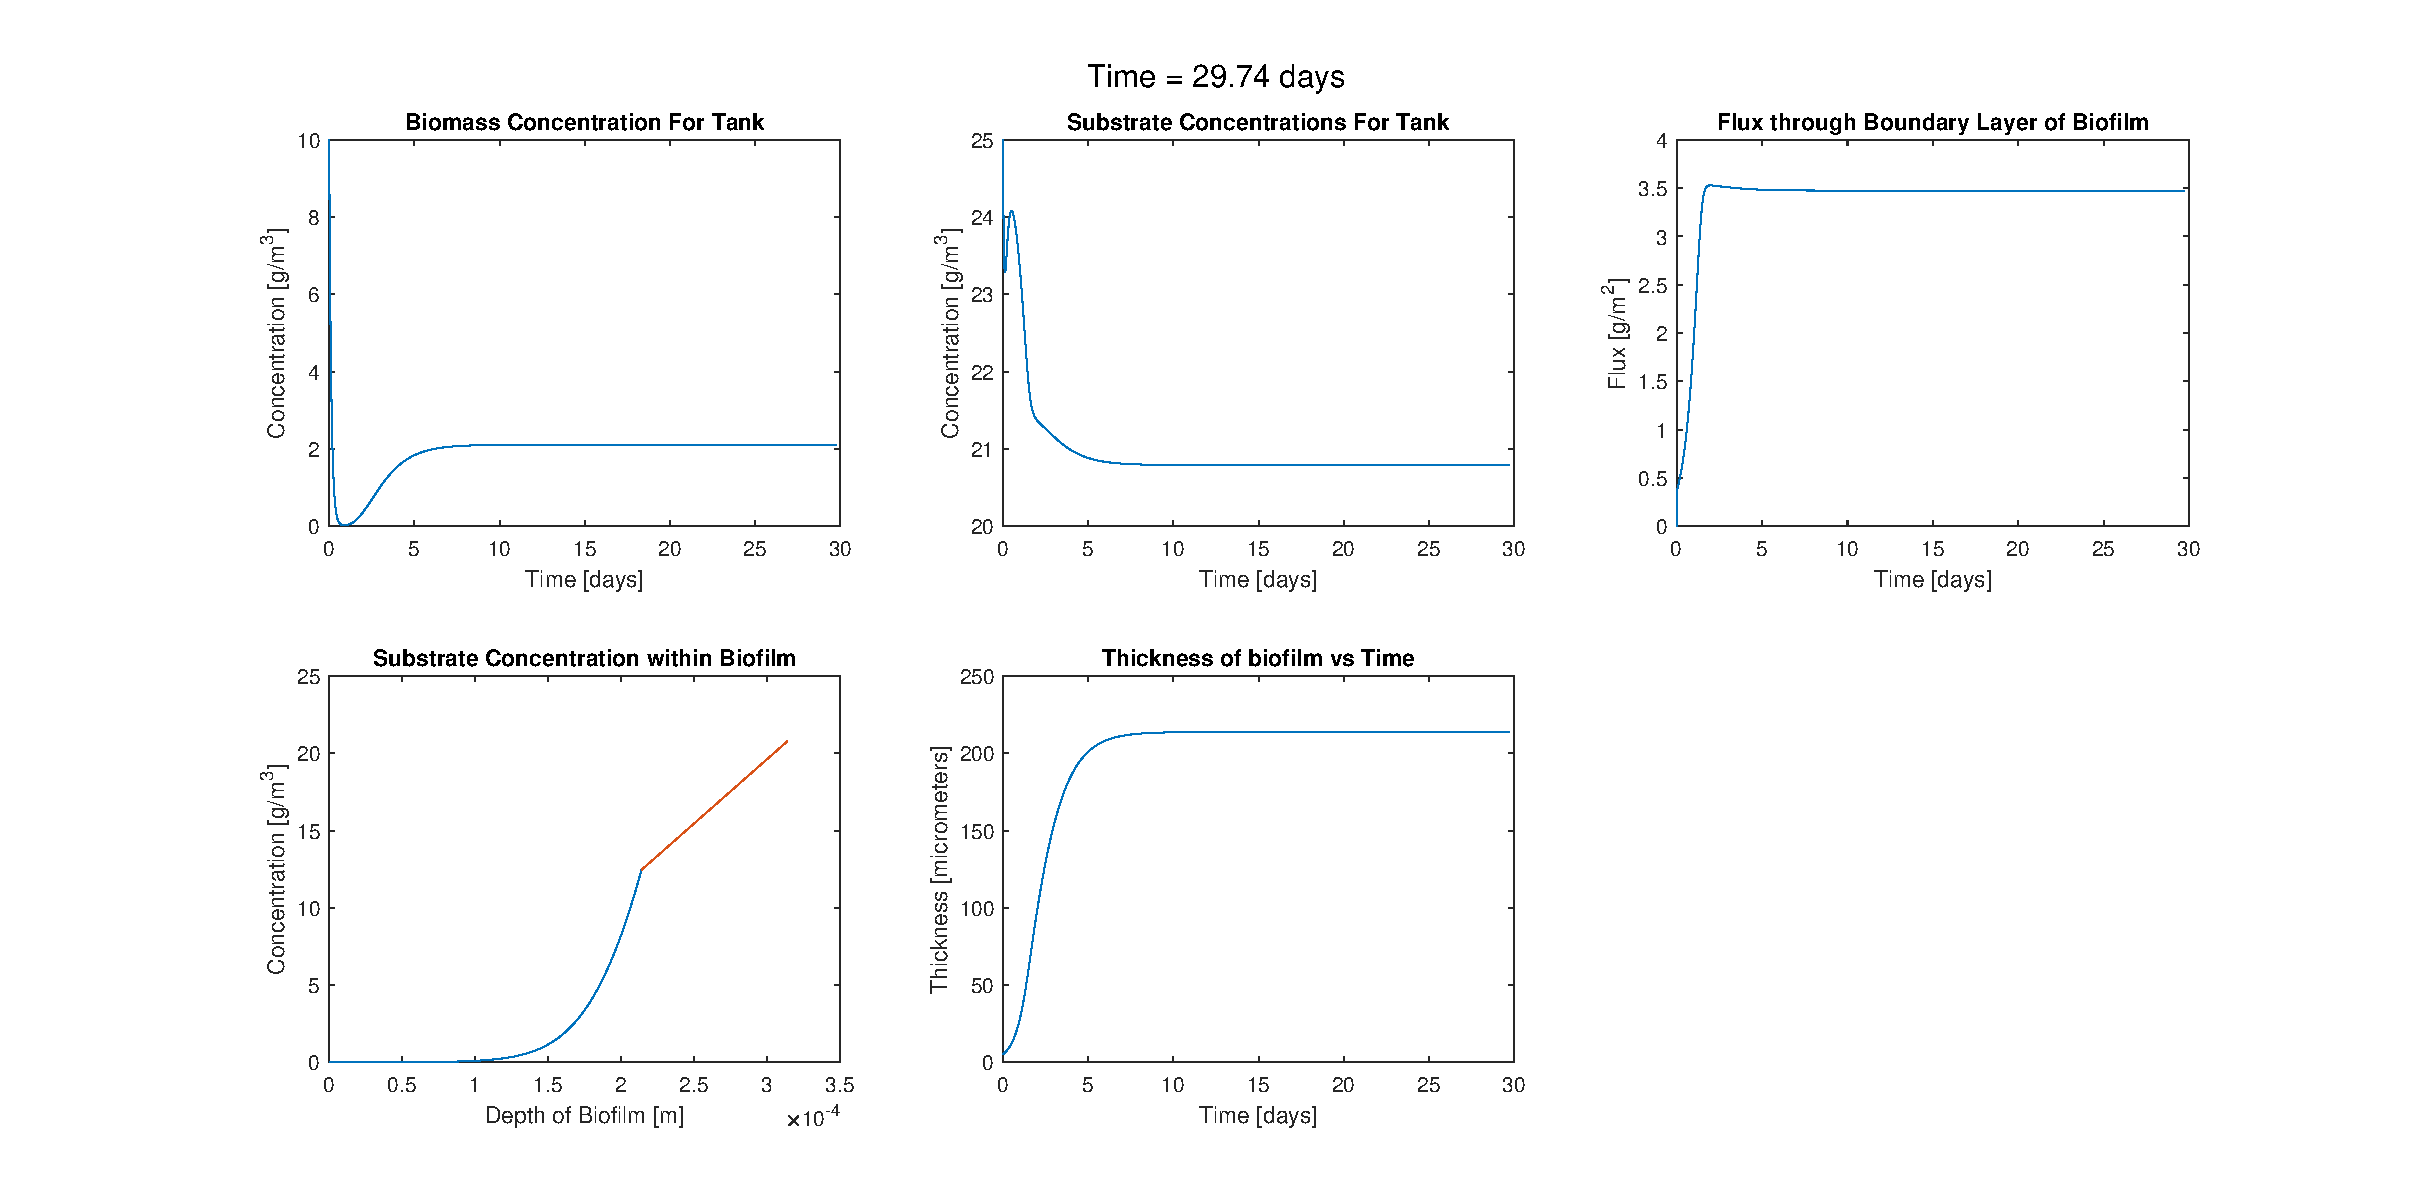
\includegraphics[read=eps, width=4in]{Testcase3_figure.eps}
  \caption{Case 3: Minimum Growth Rate Mumax}
\end{figure}

\begin{figure}[H]
  \centering
  \includegraphics[read=eps, width=4in]{Testcase4_figure.eps}
  \caption{Case 4: Elevated Inflow Q into CSTR}
\end{figure}

\section{Unit Tests for Validity}
In order to determine the accuracy of the methods and equations used in this model, unit tests were created to verify results produced by this model. This almost always involved solving a portion of the problem with a certain set of parameters so that an analytical solution could be obtained for the same problem. The following is a collection of the tests created.

\subsection{Test for when LL=0}
The purpose of this test is to show that no error occurs in the code as the boundary layer thickness goes to zero ($L_L=0$), as well as to ensure that the physics of the problem perform as expected in this case scenario.

When the boundary layer thickness goes to zero the substrate concentration at the top of the biofilm should match the substrate concentration in the tank at the given time-step. This is because without a concentration boundary layer at the top of the biofilm ($L_L=0$) diffusion of substrate into the biofilm occurs directly from the bulk fluid. In which case the flux matching boundary conditions at the top of the biofilm dealt with in section \ref{Boundary Conditions} simplify so that $S_{b,N_z}=S$ as can be seen by plugging in values to Eq.~\ref{eq:BC2_dis2}.

Parameters from case 1 are utilized to create a set of variables sufficient to run the biofilm diffusion portion of the code with two exceptions, the bulk fluid concentration $S=10$ $g/m^3$ and $L_L=0$. A grid size $N_z=50$ is applied and a linear profile of substrate concentration. It is confirmed that $S_{b,N_z}=S$ in this test within an allowable tolerance of $1E-15$. Results are visualized in the figure below.

\begin{figure}[H]
  \centering
  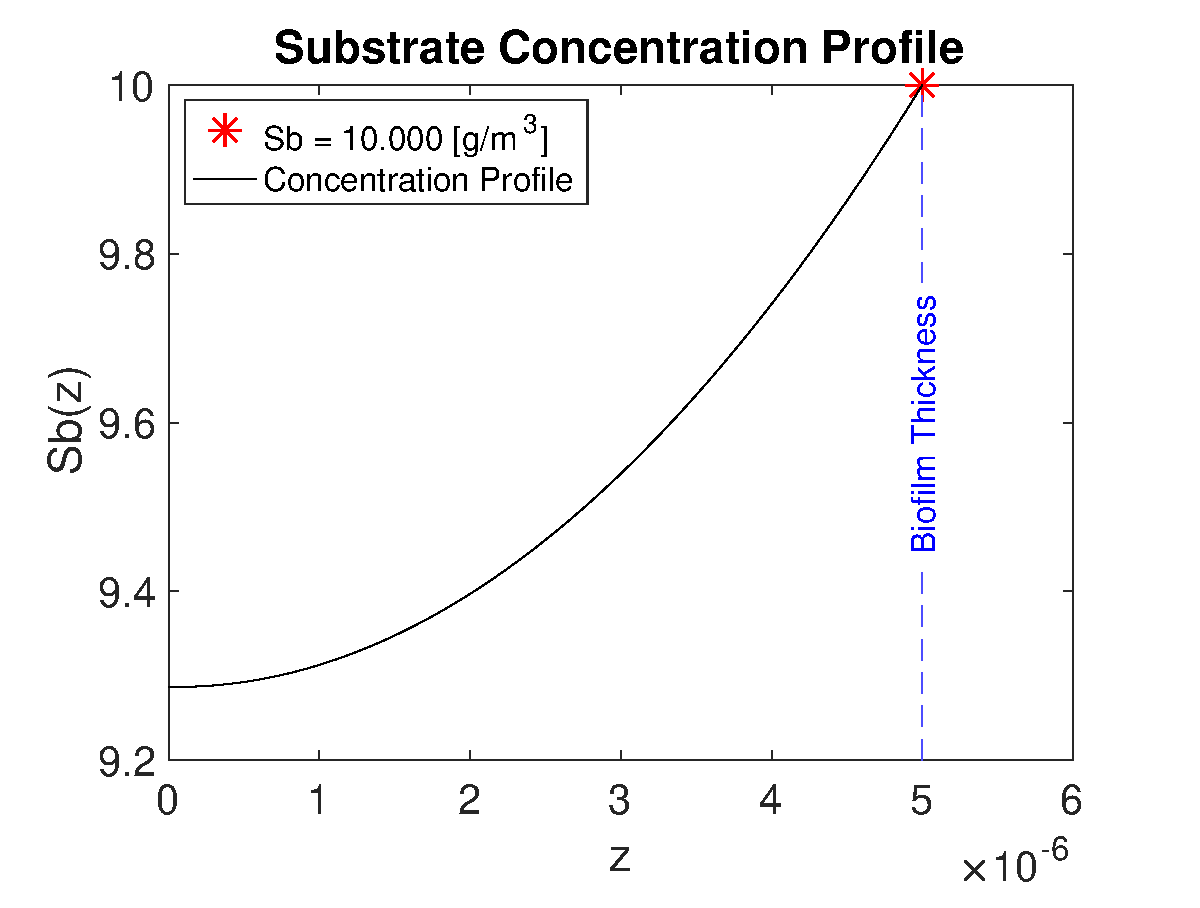
\includegraphics[read=eps, width=3in]{BoundaryLayer_Figure1.eps}
  \caption{Substrate concentration profile throughout the thickness of the biofilm.}
\end{figure}

\subsection{Test for Tank Biomass Concentration when no Inflow Q}
This is the first of three tests created to establish the validity of the 4th Order Runge-Kutta Method used to solve for the tank biomass and substrate concentrations. This test focuses on the biomass concentration. It takes equation~\ref{eq: BiomassEquation} and sets $Q=0$, establishing no inflow of biomass or substrate and eliminating said term from the differential equation. 

This test also sets $B_\mathrm{flux}=0$ in order to eliminate the diffusion of biomass into the biofilm. 
When there is no inflow and no diffusion into the biofilm, the biomass within the tank is expected to remain at its initial state, $x_o$. This is verified by the following lines of code,

\begin{lstlisting}
[~,~,x,~,~]=tankenvironment(t,x,S,Vdet,dt,bflux,param);
actSolution=x;
expSolution=xo;
tol=1e-1;
verifyLessThan(testCase,abs(actSolution-expSolution),tol);
\end{lstlisting}

These lines of code verify that the result which the code produces matches the expected analytic result to a specified tolerance.

\subsection{Test for Tank Substrate Concentration when no Inflow Q}
This test aims to replicate the previous test for the substrate concentration within the tank. When there is no inflow $Q$ of substrate, nor any substrate diffusing into the biofilm, it is expected to remain at its initial value, $S_o$. This test is verified by the following lines of code, which look very similar to the previous test.

\begin{lstlisting}
[~,~,~,S,~]=tankenvironment(t,x,S,Vdet,dt,bflux,param);
actSolution=S; 
expSolution=So;
tol=1 E-1;
verifyLessThan(testCase,abs(actSolution-expSolution),tol); 
\end{lstlisting}

Again, when the code is producing results which match the expected analytic solution to a tolerance, it can be verified that the low order Runge-Kutta Method is implemented correctly.

\subsection{Test Diffusion}
To ensure the biofilm diffusion function was operating properly with respect to the the physical situation at hand, a test was setup in which the analytical solution for substrate concentrations throughout the biofilm would be compared to those computed numerically in the biofilm diffusion function.

An analytical solution was able to be created for the substrate concentration gradient within the biofilm by enlarging parameters $\mu$ and $K_m$ in the code simulation so that external mass transfer is essentially eliminated and the tank concentration $S$ is forced to a fixed value in the bulk fluid. This analytical solution for substrate concentrations within the biofilm was computed at each location z within the biofilm with the assumptions that $\mu={S}{\mu_\mathrm{max}}$ and the boundary layer thickness $L_L=0$ with the following expression.

\begin{align}
{S_{b,\mathrm{ana}}}=\frac{S{\cosh(\frac{{\phi}{z}}{Lf})}}{\cosh(\phi)}\\
\text{where}{\quad} {\phi}=\frac{\mu_{max}{X_b}{L_f^{2}}}{{D_e}{K_m}{Y_{xs}}}
\end{align}

This test was completed for 5 different grid sizes of biofilm. Convergence of the substrate concentrations for the analytical and numerical methods can be seen as the grid size grows. The results are displayed in the figure below

\begin{figure}[H]
  \centering
  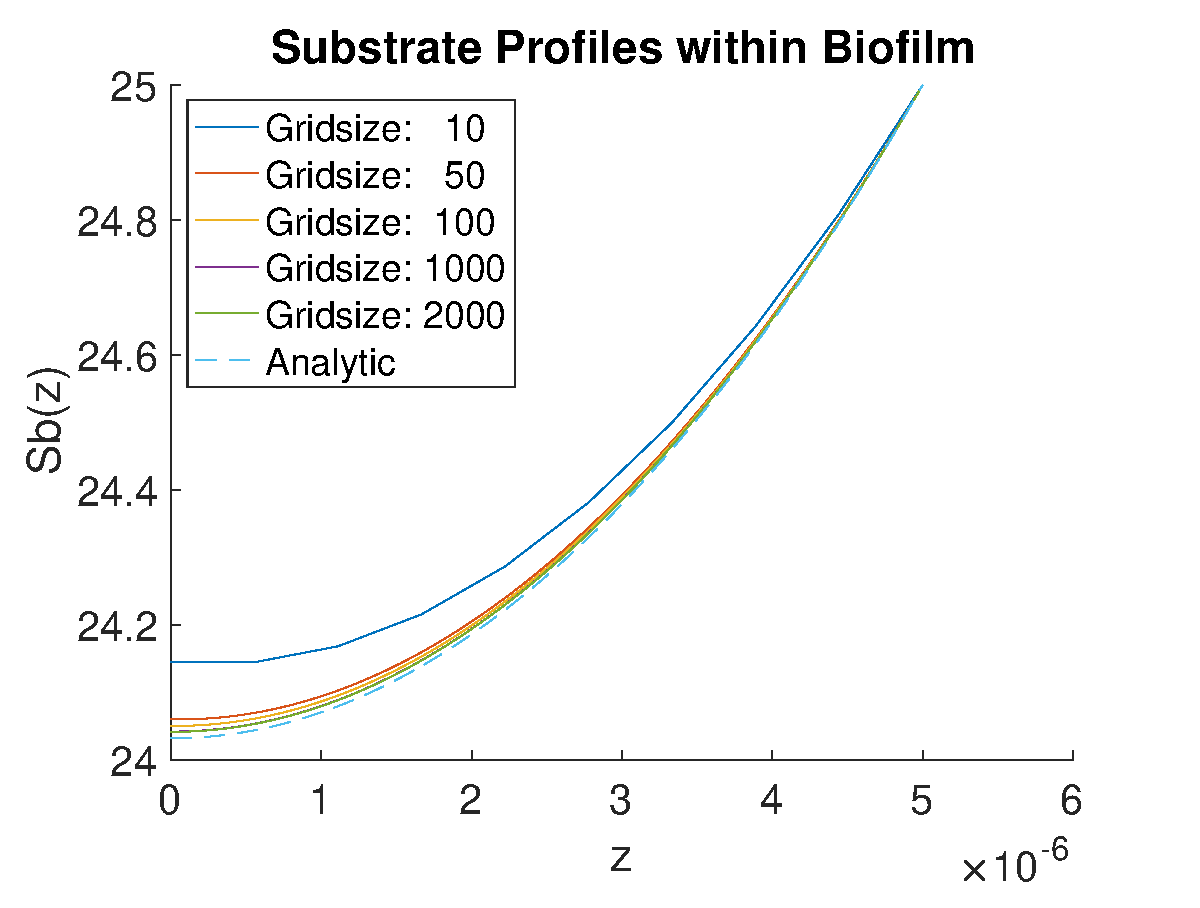
\includegraphics[read=eps, width=3in]{BiofilmDiffusion_Figure1.eps}
  \caption{Substrate concentration profiles within the biofilm for different biofilm grid sizes and the analytical expression.}
\end{figure}

\subsection{Test Steady-State with Large Diffusivities such that Substrate Concentration is Relatively Constant}

Due to the complexity of the overall biofilm problem, it is impossible to come up with an analytical solution of many parameters to check the accuracy of the code. However, by altering certain parameters within the governing equations, a hypothetical situation can be created that can be solved analytically for.

This was done by increasing the diffusion coefficients $D_e$ and $D_{aq}$ to unrealistically high levels. This in turn causes the readily available substrate present to diffuse rapidly into the biofilm, leading to a nearly uniform substrate concentration through the thickness of the biofilm at each points in time. An extremely small gradient is produced by the code in this situation as can be seen in the figure below.

\begin{figure}[H]
  \centering
  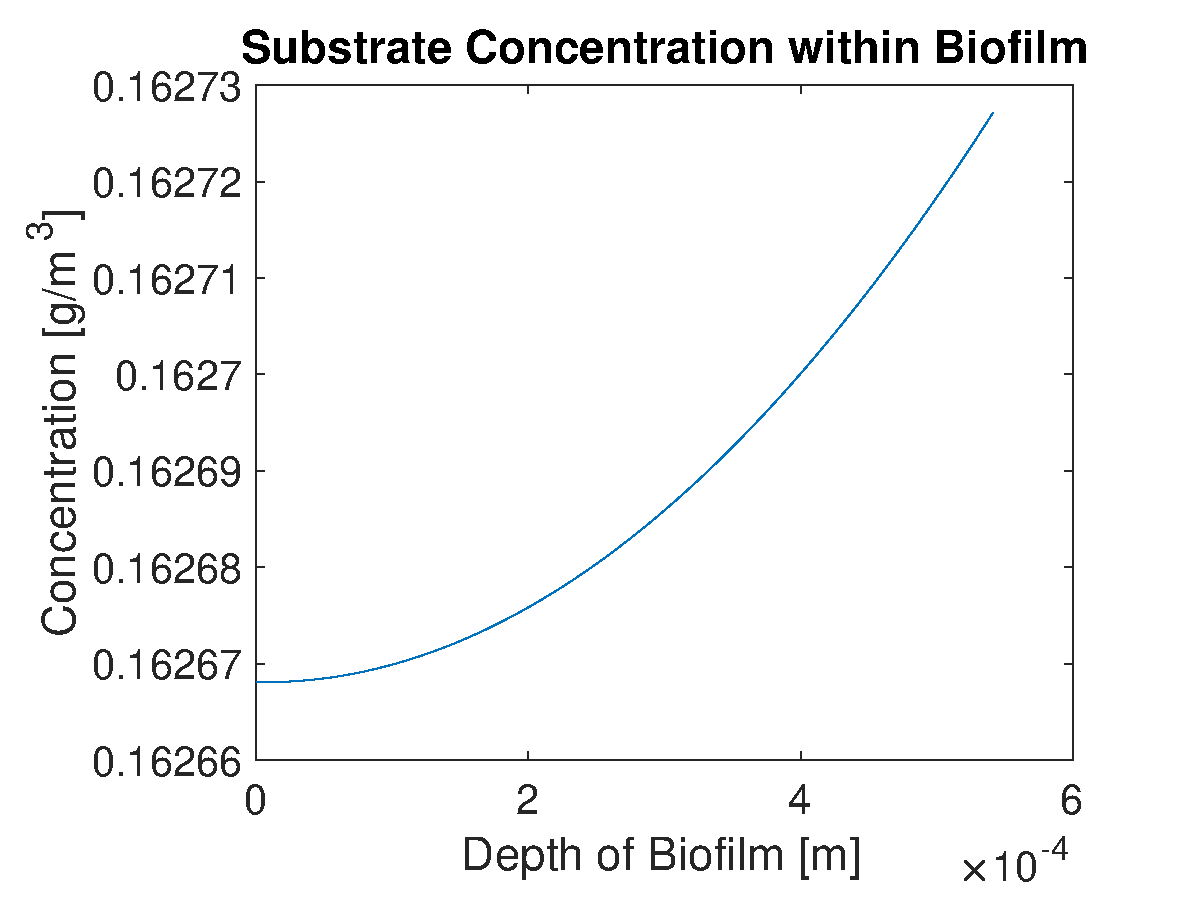
\includegraphics[read=eps, width=3in]{SteadyState_Figure1.eps}
  \caption{A depiction of the very small substrate concentration gradient within the biofilm under the given conditions.}
\end{figure}

The equations used to solve for the steady state solutions of this problem are described in \ref{Steady State}. These equations were solved iteratively within the test. The solutions produced by the code were compared to the iterative solutions found by analyzing this steady state problem. The error between each parameter was confirmed to be less than $1\%$.

\begin{center}
\begin{tabular}{ | c | c | c | } 
\hline
 \textbf{Variable} & \textbf{Steady State Solution} & \textbf{Code Solution} \\ 
 \hline
 S [{$g/m^3$}]  & 0.162686253310 & 0.162726176774 \\ 
 \hline
 x  [{$g/m^3$}] & 12.418656873345 & 12.418635483884 \\
 \hline
 Lf  [{$\mu m$}] & 541.465937430183 & 541.457821739766 \\
\hline
\end{tabular}
\end{center}


\subsection{Test Variable Time Dynamic of Tank Environment Calculations}
The low order Runge-Kutta Method used in the Matlab 'tankenvironment' function utilizes an additional 'error' step which compares the coefficients calculated to the coefficients of the Butcher Tableau. This is done to ensure that the numerical method never varies from the analytic solution beyond a certain tolerance. This error term is coupled to the time-step size term $dt$ so that maximum accuracy is obtained. 

This coupling establishes the boundaries of the allowable step size, so that that when the error is too large, the step size can shrink and reduce the inaccuracy. When the error is small, the step size can be increased to expedite the solving and improve efficiency. 

This test analyzes this operation by comparing a simplified model of the substrate environment to its corresponding analytic solution. This simulated model eliminates the biomass within the tank as well as any initial substrate concentration and profiles the development of the substrate until it reaches steady state. The analytic solution used is,
\begin{equation} \label{eq: S_ana}
  S_\mathrm{ana}=S_\mathrm{in}{(1-e^{\frac{-Q}{V}t})} + S_o
\end{equation}

If the simulated and analytic methods converge, it can be determined that the time step is properly adjusting to the magnitude of the error calculated at each point. This convergence is determined by the following lines.

\begin{lstlisting}
maxError=max(abs(S-Sana));
expTol=param.ttol;
verifyLessThan(testCase,maxError,expTol);
\end{lstlisting}

If the simulated and analytic methods produce results which match according to an established tolerance, the test will pass. Below is the plot produced which shows the convergence of simulation to analytic.

\begin{figure}[H]
  \centering
  \includegraphics[read=eps, width=3in]{TimeDynamics_Figure.eps}
  \caption{Substrate concentration profile within tank vs. time to show time-step matching.}
\end{figure}

\section{Appendix A: Steady State Behavior Test Case}\label{Steady State}

If the diffusion coefficients $D_e$ and $D_{aq}$ are considered to be very large, a steady state solution to the biofilm model can be created since full penetration of substrate into the biofilm can be assumed due to the rapid diffusion that would be occurring. In this case scenario the substrate concentration is a constant within the tank and biofilm.

The governing expressions for the biofilm may now be modified and solved for steady state for each portion of the problem as follows.

\subsection{Biofilm Thickness}
The thickness of the biofilm described by equation~\ref{eq:dLfdt_1} at steady state reduces to 

\begin{equation*}
   {\bar\mu(S_b) L_f}={k_{\mathrm{det}}L_f^2}.
\end{equation*}
 
 or by simplifying further
 
 \begin{equation}
  \label{eq:Lfsteady}
  {L_f}=\frac{\bar\mu(S_b)}{k_{\mathrm{det}}}
\end{equation}

\subsection{Biomass Concentration in Tank}
Biomass in the tank described by equation~\ref{eq: BiomassEquation}. 

\begin{equation*} 
  Qx = \mu(S) xV +v_{\mathrm{det}} A X_b
\end{equation*}
and by plugging in $v_{\mathrm{det}}= K_\mathrm{det} L_f^2 = \mu(S) L_f$ from the description of equation~\ref{eq:dLfdt_1} the following is obtained
\begin{equation}
 \label{eq:biomass steady}
  Qx = \mu(S) xV +\mu(S) L_f A X_b
\end{equation}

\subsection{Substrate Concentration}
Using the definition of $B_{\mathrm{flux}}$ from equation~\ref{eq:Bflux}, the substrate concentration in the tank described by equation~\ref{eq: SubstrateEquation} can be written as

\begin{equation}
  \frac{dS}{dt} = -\frac{\mu(S) x }{Y_{xs}} + \frac{Q S_{\mathrm{in}}}{V} - \frac{Q S}{V} -\frac{\bar\mu(S_b) X_b V_b}{Y_{xs}{V}}
\end{equation}

where $V_b=A L_f$ is the volume of the biofilm.  At steady-state this simplifies to 
\begin{equation}
 \label{eq:x steady}
   x = \frac{Y_{xs}}{\mu V}\left(Q S_{\mathrm{in}} - Q S\right) -\frac{\bar{\mu} V_b}{\mu V}{X_b}
\end{equation}

\subsection{Solving for Steady State Parameters}
Equation~\ref{eq:Lfsteady},~\ref{eq:biomass steady}, and~\ref{eq:x steady} were defined in Matlab. From here an initial guess of $S$ is made. $S$ is increased incrementally in a loop until the right hand side equals the left hand side of equation~\ref{eq:biomass steady} to within a tolerance of $1E-12$.

\end{document}